\documentclass[a4paper]{article}

\usepackage{INTERSPEECH2022}

% Replace the title below with something more specific if you wish
\title{A face verification system}

% Replace the 'ac1jpb' with your username
\name{ac1jpb}

% Please do not use your actual name. We prefer to mark work anonymously.

\address{University of Sheffield}

\begin{document}

\maketitle

% Lines starting with a percent symbol are comments.
%
% The text in this paper is just dummy text so that you can get an idea of what the final report will look like. Delete it and replace it with your report's content.
%
% The final paper should not be any longer than 2-sides of A4.
% The word count is not expected to be more than 1200 words.

\begin{abstract}
   % The text for your abstract goes here. The abstract should summarise the paper and be no more than about 100 words

   Lorem ipsum dolor sit amet, consectetur adipiscing elit. Proin sagittis lacus velit. Phasellus sodales sed ipsum eget mollis. Quisque et cursus ex. Etiam quis libero quis magna fermentum vehicula sed suscipit eros. Etiam eu dictum augue. Etiam tempor et eros in condimentum. In non convallis nulla. Vestibulum volutpat risus vel commodo sagittis. Aliquam erat volutpat. Ut ac consectetur justo. Vivamus interdum cursus diam, ac convallis arcu efficitur non. Maecenas odio elit, finibus porta risus tempus, tristique faucibus lorem. Donec placerat, odio sed auctor lacinia, tellus magna dignissim sapien, accumsan consectetur velit massa quis eros. Maecenas et lectus et neque commodo pharetra.

\end{abstract}

\section{Introduction}

% The introduction should briefly describe the face verification problem
% that you are trying to solve.
%
% End the introduction by providing a short overview of the rest of the report.

Lorem ipsum dolor sit amet, consectetur adipiscing elit. Fusce consequat ante eu quam mattis commodo. Vivamus pretium vitae nibh eget porta. Nulla sollicitudin euismod mauris non convallis. Praesent blandit purus blandit posuere ullamcorper. Integer sed pulvinar sapien. Praesent vehicula urna nec sollicitudin suscipit. Sed facilisis augue eu augue gravida, eu hendrerit neque laoreet. Integer porttitor tincidunt lacinia. Suspendisse non arcu viverra, dictum mauris quis, malesuada nisi. Donec neque enim, molestie id ornare id, finibus sed felis. Donec venenatis condimentum orci, aliquam consequat dui sagittis imperdiet. Curabitur ut varius enim. Ut vel risus et urna sollicitudin condimentum. Suspendisse gravida dui mollis diam varius, vel tristique libero feugiat.

Proin a ante molestie, mollis ipsum ut, posuere enim. Aenean cursus tellus vitae enim fringilla, a finibus nibh dictum. Maecenas convallis est in libero fringilla, id pharetra purus fermentum. Donec dignissim, ligula vel mattis volutpat, metus nisi pulvinar nunc, ut pharetra urna ex quis urna. Curabitur egestas lacus erat, eget convallis sem eleifend eget. Donec luctus, quam vitae pharetra scelerisque, ligula lorem placerat lectus, nec hendrerit tortor nisi nec nulla. Nunc non pellentesque sapien, et consectetur orci. Vestibulum et porttitor lacus. Proin dapibus rutrum egestas. Proin congue mattis sem, tempor laoreet felis mattis ac.


\section{System Description}

% This section should describe your complete system in detail.
% Try and describe it in sufficient detail such that other can replicate your results.
% The complete system includes all the steps from inputting the image-pair to get out the classification result, i.e., it will include all the steps in your processing pipeline.
% In particular, highlight any hyper-parameters that you will tune when you run your experiments.

Lorem ipsum dolor sit amet, consectetur adipiscing elit. Cras lobortis, elit id congue accumsan, elit dui pharetra mi, eu consequat ligula nulla ut lorem. Nulla quis massa ultricies, auctor libero id, porttitor augue. Donec purus nunc, accumsan ut nisi non, lacinia tempor turpis. Donec lorem arcu, consectetur et sollicitudin in, pretium sed risus. Nam pharetra sapien dui. Nunc vitae felis turpis. Pellentesque non elit sed tellus suscipit laoreet. Nulla facilisi. Integer molestie urna in mollis hendrerit. Proin non hendrerit tellus.

Aenean non enim id purus sagittis cursus eu vitae sem. Curabitur sagittis sapien vitae lorem blandit, non venenatis lacus vulputate. Maecenas quis massa quis nunc tempor viverra. Donec pharetra lacinia lobortis. Vestibulum lectus magna, vestibulum id molestie a, ornare in sem. Morbi vel facilisis lectus. Vestibulum porta vehicula sapien a ultricies. Nam dignissim rhoncus odio, vitae blandit lacus pharetra vel. Morbi luctus quam ac venenatis placerat. Nunc convallis, risus et vestibulum cursus, urna lorem viverra justo, a congue ipsum odio a felis.

In sit amet est et nunc maximus pulvinar non vel magna. Vestibulum facilisis ante id est dictum malesuada at at augue. Pellentesque condimentum justo nec orci faucibus pharetra. Integer malesuada tristique malesuada. Integer pellentesque nisl nec justo scelerisque, eget dictum purus volutpat. Mauris sodales, libero quis vestibulum tempor, sapien dolor tincidunt nulla, a mattis purus metus eu magna. Nunc viverra molestie erat et commodo. Cras auctor dui ac ante interdum, eget finibus mauris imperdiet. Nulla ullamcorper magna nec nibh viverra congue nec volutpat diam. Nunc eget lacus tincidunt, elementum leo eu, maximus odio. Etiam pharetra viverra cursus. Cras blandit elit a euismod ultrices. Nunc vulputate, dolor in mattis consectetur, felis justo rutrum diam, in mollis elit eros facilisis tellus. Cras quis pulvinar odio. In finibus consequat dignissim. Nulla vel velit a dui bibendum varius ac non odio. Nulla.

\section{Experiments}

% Describe the experiments that you have conducted to optimise the performance of your system.
% For example,
%  - How did you choose the best training data.
%  - How did you optimise your systems hyperparameters.
%  - How did you ensure that you didn't exceed the allowed model size.
% You can include results in this section, e.g. results obtained when trying different hyper-parameter settings.

Lorem ipsum dolor sit amet, consectetur adipiscing elit. Cras lobortis, elit id congue accumsan, elit dui pharetra mi, eu consequat ligula nulla ut lorem. Nulla quis massa ultricies, auctor libero id, porttitor augue. Donec purus nunc, accumsan ut nisi non, lacinia tempor turpis. Donec lorem arcu, consectetur et sollicitudin in, pretium sed risus. Nam pharetra sapien dui. Nunc vitae felis turpis. Pellentesque non elit sed tellus suscipit laoreet. Nulla facilisi. Integer molestie urna in mollis hendrerit. Proin non hendrerit tellus.

Aenean non enim id purus sagittis cursus eu vitae sem. Curabitur sagittis sapien vitae lorem blandit, non venenatis lacus vulputate. Maecenas quis massa quis nunc tempor viverra. Donec pharetra lacinia lobortis. Vestibulum lectus magna, vestibulum id molestie a, ornare in sem. Morbi vel facilisis lectus. Vestibulum porta vehicula sapien a ultricies. Nam dignissim rhoncus odio, vitae blandit lacus pharetra vel. Morbi luctus quam ac venenatis placerat. Nunc convallis, risus et vestibulum cursus, urna lorem viverra justo, a congue ipsum odio a felis.

In sit amet est et nunc maximus pulvinar non vel magna. Vestibulum facilisis ante id est dictum malesuada at at augue. Pellentesque condimentum justo nec orci faucibus pharetra. Integer malesuada tristique malesuada. Integer pellentesque nisl nec justo scelerisque, eget dictum purus volutpat. Mauris sodales, libero quis vestibulum tempor, sapien dolor tincidunt nulla, a mattis purus metus eu magna. Nunc viverra molestie erat et commodo. Cras auctor dui ac ante interdum, eget finibus mauris imperdiet. Nulla ullamcorper magna nec nibh viverra congue nec volutpat diam. Nunc eget lacus tincidunt, elementum leo eu, maximus odio. Etiam pharetra viverra cursus. Cras blandit elit a euismod ultrices. Nunc vulputate, dolor in mattis consectetur, felis justo rutrum diam, in mollis elit eros facilisis tellus. Cras quis pulvinar odio. In finibus consequat dignissim. Nulla vel velit a dui bibendum varius ac non odio. Nulla.

Lorem ipsum dolor sit amet, consectetur adipiscing elit. Cras lobortis, elit id congue accumsan, elit dui pharetra mi, eu consequat ligula nulla ut lorem. Nulla quis massa ultricies, auctor libero id, porttitor augue. Donec purus nunc, accumsan ut nisi non, lacinia tempor turpis. Donec lorem arcu, consectetur et sollicitudin in, pretium sed risus. Nam pharetra sapien dui. Nunc vitae felis turpis. Pellentesque non elit sed tellus suscipit laoreet. Nulla facilisi. Integer molestie urna in mollis hendrerit. Proin non hendrerit tellus.

Aenean non enim id purus sagittis cursus eu vitae sem. Curabitur sagittis sapien vitae lorem blandit, non venenatis lacus vulputate. Maecenas quis massa quis nunc tempor viverra. Donec pharetra lacinia lobortis. Vestibulum lectus magna, vestibulum id molestie a, ornare in sem. Morbi vel facilisis lectus. Vestibulum porta vehicula sapien a ultricies. Nam dignissim rhoncus odio, vitae blandit lacus pharetra vel.

\section{Results and Analysis}

% Here you should report the results obtained on the evaluation data with your final system.
%
% You can also analyse the performance. For example, you may want to look at cases where it is failing
% and try to understand the conditions that lead to these failures.

Lorem ipsum dolor sit amet, consectetur adipiscing elit. Cras lobortis, elit id congue accumsan, elit dui pharetra mi, eu consequat ligula nulla ut lorem. Nulla quis massa ultricies, auctor libero id, porttitor augue. Donec purus nunc, accumsan ut nisi non, lacinia tempor turpis. Donec lorem arcu, consectetur et sollicitudin in, pretium sed risus. Nam pharetra sapien dui. Nunc vitae felis turpis. Pellentesque non elit sed tellus suscipit laoreet. Nulla facilisi. Integer molestie urna in mollis hendrerit. Proin non hendrerit tellus.

Aenean non enim id purus sagittis cursus eu vitae sem. Curabitur sagittis sapien vitae lorem blandit, non venenatis lacus vulputate. Maecenas quis massa quis nunc tempor viverra. Donec pharetra lacinia lobortis. Vestibulum lectus magna, vestibulum id molestie a, ornare in sem. Morbi vel facilisis lectus. Vestibulum porta vehicula sapien a ultricies. Nam dignissim rhoncus odio, vitae blandit lacus pharetra vel. Morbi luctus quam ac venenatis placerat. Nunc convallis, risus et vestibulum cursus, urna lorem viverra justo, a congue ipsum odio a felis.

Aenean non enim id purus sagittis cursus eu vitae sem. Curabitur sagittis sapien vitae lorem blandit, non venenatis lacus vulputate. Maecenas quis massa quis nunc tempor viverra. Donec pharetra lacinia lobortis. Vestibulum lectus magna, vestibulum id molestie a, ornare in sem. Morbi vel facilisis lectus. Vestibulum porta vehicula sapien a ultricies. Nam dignissim rhoncus odio, vitae blandit lacus pharetra vel.

\section{Discussion and Conclusions}

% Briefly discuss your results and summarise conclusions.
% e.g., How well did the verification system work? How much impact did the sub-image size have on performance? How sensitive was the performance to hyperparameter tuning? If you had more time, what could be done to further increase performance?

Lorem ipsum dolor sit amet, consectetur adipiscing elit. Cras lobortis, elit id congue accumsan, elit dui pharetra mi, eu consequat ligula nulla ut lorem. Nulla quis massa ultricies, auctor libero id, porttitor augue. Donec purus nunc, accumsan ut nisi non, lacinia tempor turpis. Donec lorem arcu, consectetur et sollicitudin in, pretium sed risus. Nam pharetra sapien dui. Nunc vitae felis turpis. Pellentesque non elit sed tellus suscipit laoreet. Nulla facilisi. Integer molestie urna in mollis hendrerit. Proin non hendrerit tellus.


\section{Using Latex}

This section should not appear in your report, but has been included here so you have some examples of how to use LaTex.

\subsection{Adding citations}
A citation can be added using the cite command as follows \cite{Davis80-COP}. The parameter value passed to the command should be one of the keys from the file `mybib.bib'. For any reference that you want to cite, you will need to add a corresponding entry to the `mybib.bib' file. Citations are most likely to appear in your Background section, e.g. when describing the type of classifier that you are using.

\subsection{Figure, Tables and Equations}

This is how you reference a figure. Figure \ref{fig:face} shows a sub-image extracted from a face.

\begin{figure}[t]
    \centering
    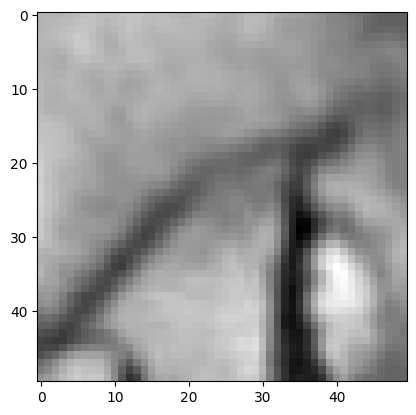
\includegraphics[width=0.8\linewidth]{face50_1.png}
    \caption{A 50 by 50 pixel sub-image sampled from a face.}
    \label{fig:face}
  \end{figure}

This is how you reference a table. Table \ref{tab:example} shows how you might present results of a hyperparameter tuning experiment.
\begin{table}[th]
    \caption{The system performance for different values of k.}
    \label{tab:example}
    \centering
    \begin{tabular}{ c|c}
      \toprule
      k & \% Correct\\
      \midrule
       1 & 94.4 \\
       3 & 95.6 \\
       5 & 96.1 \\
       7 & 95.2 \\
       9 & 94.0 \\
       11 & 92.1 \\
      \bottomrule
    \end{tabular}

  \end{table}

  LaTex makes it very easy to format equations. For example, the functional form of the univariate Gaussian Normal distribution is,

  \begin{equation}
P(x) = \frac{1}{\sigma \sqrt {2\pi } }e^{\frac{ - \left( {x - \mu } \right)^2 }{2\sigma^2}}
\label{eq:gaussian}
  \end{equation}



% Do not touch any lines below here
\bibliographystyle{IEEEtran}
\bibliography{mybib}

\end{document}
